%% LyX 1.1 created this file.  For more info, see http://www.lyx.org/.
%% Do not edit unless you really know what you are doing.
\documentclass[english]{amsart}
\usepackage[T1]{fontenc}
\usepackage[latin1]{inputenc}
\usepackage{babel}
\usepackage{graphics}

\makeatletter

%%%%%%%%%%%%%%%%%%%%%%%%%%%%%% LyX specific LaTeX commands.
\providecommand{\LyX}{L\kern-.1667em\lower.25em\hbox{Y}\kern-.125emX\@}

%%%%%%%%%%%%%%%%%%%%%%%%%%%%%% Textclass specific LaTeX commands.
 \theoremstyle{plain}    
 \newtheorem{thm}{Theorem}[section]
 \numberwithin{equation}{section} %% Comment out for sequentially-numbered
 \numberwithin{figure}{section} %% Comment out for sequentially-numbered
 \theoremstyle{plain}    
 \newtheorem{lem}[thm]{Lemma} %%Delete [thm] to re-start numbering
 \theoremstyle{plain}    
 \newtheorem{prop}[thm]{Proposition} %%Delete [thm] to re-start numbering

%%%%%%%%%%%%%%%%%%%%%%%%%%%%%% User specified LaTeX commands.
\newcommand{\R}{{\sf R\hspace*{-0.9ex}\rule{0.15ex}%
       {1.3ex}\hspace*{0.9ex}}}
\newcommand{\N}{{\sf N\hspace*{-1.0ex}\rule{0.15ex}%
       {1.1ex}\hspace*{1.0ex}}}
\newcommand{\Q}{{\sf Q\hspace*{-1ex}\rule{0.15ex}%
       {1.3ex}\hspace*{1.1ex}}}
\newcommand{\C}{{\sf C\hspace*{-0.9ex}\rule{0.15ex}%
       {1.3ex}\hspace*{0.9ex}}}
\usepackage{epsfig}
\usepackage{amsmath,amssymb}
\usepackage{pslatex}
\usepackage{color}
 
 \definecolor{veryblackblue}{rgb}{0.0,0.0,0.1}
 


\topmargin  = 0pt
\headheight = 0pt
\headsep    = 0pt

\voffset    = 0in
\hoffset    = 0in
\textheight = 230mm
\textwidth  = 164mm

\evensidemargin = 0pt
\oddsidemargin  = 0pt

\pagestyle{empty}
\usepackage{float}

%% Background of blue palette
 \definecolor{webblackblue}{rgb}{0.0,0.0,0.2}
 \definecolor{webblue}{rgb}{0.0, 0.0, 0.6}

%% Background of red palette
 \definecolor{webblackred}{rgb}{0.2,0.0,0.0}
 \definecolor{webred}{rgb}{0.6,0.0,0.0}

%% Background of green palette
 \definecolor{webblackgreen}{rgb}{0.0,0.2,0.0}                                   
 \definecolor{webgreen}{rgb}{0.0,0.6,0.0} 

%% Background of magenta palette
 \definecolor{webblackmagenta}{rgb}{0.14,0.0,0.14}                                   
 \definecolor{webmagenta}{rgb}{0.42,0.0,0.42} 

%% Background of cyan palette
 \definecolor{webblackcyan}{rgb}{0.0,0.14,0.14}                                   
 \definecolor{webcyan}{rgb}{0.0,0.42,0.42} 

%% Background of yellow pallete
 \definecolor{webblackyellow}{rgb}{0.14,0.14,0.0}                                   
 \definecolor{webyellow}{rgb}{0.85,0.85,0.0} 

 \definecolor{webdarkgray}{rgb}{0.2,0.2,0.2}

 \definecolor{webgray}{rgb}{0.75,0.75,0.75}
 \definecolor{weborange}{rgb}{1.0, 0.6, 0.0}

\renewcommand\labelenumi{\textcolor{webdarkgray}{\arabic{enumi}.}}
\newcommand{\setenumi}[1]{#1.\setcounter{enumi}{#1}}
\usepackage{dsfont}

\makeatother
\begin{document}

\title{A family of 4-point dyadic high resolution subdivision schemes}

\maketitle

\section{ntroduction}

Interpolatory subdivision schemes interpolate a discrete set of data
points in a local manner, that is, the value of the interpolation
function at a given point depends on a small number of nearby data
points. The classical dyadic algorithm introduced by Deslauriers and
Dubuc finds the midpoint values by fitting a Lagrange polynomial through
the \( 2N \) closest data points. By repeating this algorithm again
and again, each time doubling the number of data points or nodes,
we eventually have a dense set of data points and we can determine
uniquely a smooth interpolation function. 

This type of approach is very convenient to implement in software
and the fact that subdivision schemes are strictly local makes them
robust. They also inherit their order of approximation from the corresponding
Lagrange interpolation scheme. Because interpolatory subdivision schemes
relate data points from one scale to the data points at another scale,
it is not surprising that they are a key ingredient in the construction
of compactly supported wavelets .

Since Deslauriers-Dubuc schemes have important applications, it is
tempting to add extra nodes to Deslauriers and Dubuc schemes as an
attempt to improve them to get {}``high resolution'' schemes. One
might hope to retain the useful properties such as the approximation
order and the regularity while making the scheme more local for example.
Doubling the number of nodes however is costly (effectively doubling
the memory requirements), however, since a dyadic subdivision scheme
doubles its memory usage at each step, we can choose to use right
away this upcoming extra storage space without any cost. In effect,
we can simply make use of the memory we will allocate later in any
case. Therefore, we can double (or more) the number of nodes. These
new placeholders can then be used to record a first coarse scale guess
(using a tetradic filter) which we can later combine with a finer
scale interpolation (using a dyadic filter) . As a special case, we
may choose to ignore the coarse scale estimate, in which case our
approach amounts to a Deslauriers-Dubuc scheme; we can also use this
approach to reproduce polynomials of degree \( 4 \) by a Richardson
extrapolation approach. This paper shows that by summing up the tetradic
(coarse) interpolation recorded in placeholders and dyadic (fine)
interpolations, we get a range of smooth (\( C^{1} \)) high resolutions
schemes reproducing cubic polynomials. 

In a general \( b- \)adic, we propose to extend subdivision schemes
of the form \( y_{j+1,l}=\sum _{k\in \N }\gamma _{bk-l}y_{j,k} \)
by \[
y_{j+1,l}=\sum _{m=1}^{N}\sum _{k\in \N }\gamma _{Nbk+m-1-l}^{(m)}y_{j,Nk+m-1}.\]
 In the Fourier domain, this amounts to replacing . \( P^{j+1}(z)=\Gamma (z)P^{j}(z^{b}) \)
by \( P^{j+1}(z)=\sum _{i=1}^{M}\Gamma _{i}(z)P^{j}\left( e^{2\pi i/b}z^{b}\right)  \).

\vspace{0.3cm}
{
\begin{figure}
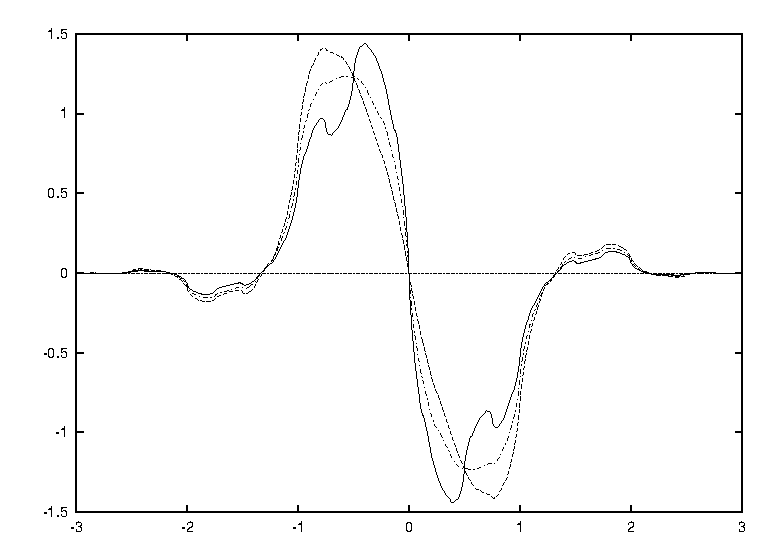
\includegraphics{firstderivative_fund_-0.2_0.15_0.eps} 


\caption{Derivatives of 3 fundamental functions for 3 different \protect\( 4-\protect \)point
cubic high resolution interpolatory subdivision schemes. The dot-dash
curve is the special case where we get the Deslauriers-Dubuc scheme.}
\end{figure}
\par}


\section{Subdivision schemes}

Interpolatory subdivision schemes where first introduced by Deslauriers
and Dubuc (quote). Let \( b>1 \) be an integer, given two integers
\( k,j \), the number \( x_{j,k}=k/b^{j} \) is said to be \( b- \)adic
(of depth \( j \)). For a fixed \( j \), the \( b- \)adic numbers
form a regularly-spaced set of nodes. Given some corresponding data
\( \left\{ y_{J,k}\right\} _{k\in \N } \) on the dyadic numbers of
depth \( J \), we want to build a smooth fonction \( f \) such that
\( f\left( x_{J,k}\right) =y_{J,k}\, \forall k\in \N  \). Starting
with this initial data (\( y_{J,k} \)) and using the linear formula
\begin{equation}
\label{basicsubdivision}
y_{j+1,l}=\sum _{k\in \N }\gamma _{bk-l}y_{j,k}
\end{equation}
 for some constant array \( \gamma  \), we get values \( y_{J,k} \)
for any \( j>J \) and since \( b- \)adic numbers form a dense set
of the real numbers, there is at most one continuous function such
that \( f\left( x_{j,k}\right) =y_{j,k} \) for all \( k,j>J \). 

A subdivision scheme is interpolatory and will satisfy \( f\left( x_{J,k}\right) =y_{J,k} \)
if \( \gamma _{bk}=0 \) except when \( k=0 \). We say that a subdivision
scheme is stationary if the array \( \gamma  \) is constant (doesn't
depend on \( j \)). An interpolatory subdivision scheme is said to
be \( 2N- \)point if \( \gamma _{l}=0 \) for \( |l|>Nb \). The
interpolation function \( f \) computed from a \( 2N- \)point \( b- \)adic
scheme with initial data \( y_{0,0}=1 \) and \( y_{0,k}=0 \) for
all \( k\neq 0 \) is said to be the fundamental function and has
a compact support of \( [-(Nb-1)/(b-1),(Nb-1)/(b-1)] \) or \( [1-2N,2N-1] \)
when \( b=2 \). Hence as \( N \) increases the support of the fundamental
function increases.

For each \( N=1,2,3,... \) there exists a corresponding an interpolatory
Deslauriers-Dubuc subdivision scheme and they are built from the midpoint
evaluation of Lagrange polynomial of degree \( 2N-1 \) on \( 2N \)
points. For \( b=2 \) (dyadic case), the \( 4- \)point Deslauriers-Dubuc
scheme can be defined by the array \( \gamma ^{DD2} \) given by \( \gamma _{0}^{DD2}=1,\,  \)\( \gamma _{1}^{DD2}=\gamma ^{DD2}_{-1}=-9/16,\,  \)\( \gamma _{3}^{DD2}=\gamma _{-3}^{DD2}=-1/16 \)
with \( \gamma _{k}^{DD2}=0 \) otherwise; for \( b=4 \) (tetradic
case), the scheme is defined by \( \gamma ^{DD4} \) given by \( \gamma _{2k}^{DD4}=\gamma ^{DD2}_{k}\, \forall k\in \N ,\,  \)
\( \gamma _{-1}^{DD4}=\gamma _{1}^{DD4}=105/128,\,  \)\( \gamma _{-3}^{DD4}=\gamma _{-3}^{DD4}=35/128,\,  \)\( \gamma _{-5}^{DD4}=\gamma _{5}^{DD4}=-7/128,\,  \)\( \gamma _{-7}^{DD4}=\gamma _{7}^{DD4}=-5/128,\,  \)with
\( \gamma _{k}^{DD2}=0 \) otherwise. Because \( 4- \)point Deslauriers-Dubuc
schemes are derived from cubic Lagrange polynomials, they reproduces
cubic polynomials, that is, if the initial data \( y_{j,k} \) satisfies
\( y_{j,k}=p\left( x_{j,k}\right) \, \forall k\in \N  \) for some
cubic polynomial \( p \) then the interpolation function \( f \)
is this same cubic polynomial \( f=p \). Hence the two cases presented
above (\( \gamma ^{DD2} \) and \( \gamma ^{DD4} \)) reproduce cubic
polynomials. It can also be shown also that they both give differentiable
(\( C^{1} \)) interpolation functions.

We are interested in measuring how well a given subdivsion scheme
can approximation functions. One such measure is given by the approximation
order of the scheme\cite[definition 2]{KuVD98}. We say that a subdivision
scheme has approximation order \( p \) if given given any smooth
function \( g\in C^{p}\left( \left[ 0,1\right] \right)  \), the interpolation
function \( f \) satisfying \( f\left( x_{j,k}\right) =g\left( x_{j,k}\right) \, \forall k\in \N  \)
is such that \( \left\Vert f-g\right\Vert _{L^{\infty }\left( \left[ 0,1\right] \right) }\leq C/2^{jp} \)
for a constant \( C \) independent of \( j \).

For a continuous subdivision scheme reproducing polynomials of degree
\( p \), it is sufficient for the scheme to converge to a continous
function to have approximation order \( p+1 \) \cite{KuVD98}. Specifically,
this means that \( 4- \)point Deslauriers-Dubuc schemes have approximation
order \( 4 \).


\section{High resolution subdivsion schemes}


\subsection{Definitions}

An more general alternative to equation \ref{basicsubdivision} is
given by the linear equation\[
y_{j+1,l}=\sum _{m=1}^{N}\sum _{k\in \N }\gamma _{Nbk+m-1-l}^{(m)}y_{j,Nk+m-1}\]
where \( \gamma ^{(1)},...,\gamma ^{(N)} \) are constant arrays (independent
from \( j \)). Because this new formula uses \( N \) times the usual
number of nodes (see equation \ref{basicsubdivision}), we say that
it is a {}``high resolution subdivision scheme'' however it can
still be said to be \( b- \)adic because the number of nodes is increasing
by \( b \). As a special case, when \( N=1 \), we have a usual subdivision
scheme. 

In what follows, we set \( b=N=2 \) and consider the equation\begin{equation}
\label{N2highres}
y_{j+1,l}=\sum _{k\in \N }\gamma _{4k-l}^{(1)}y_{j,2k}+\gamma _{4k+1-l}^{(2)}y_{j,2k+1}
\end{equation}
with \begin{eqnarray}
\gamma ^{(1)}_{k} & = & \gamma ^{DD4}_{k}-\alpha \frac{\left( (-1)^{k}+1\right) }{2}\gamma ^{DD2}_{k/2}+\alpha \delta _{k,0}\, \forall k\in \N \label{N2highres_1} \\
\gamma ^{(2)}_{0} & = & \alpha ,\, \gamma ^{(2)}_{k}=0\, otherwise\label{N2highres_2} 
\end{eqnarray}
 for some parameter \( \alpha \in \R  \). As we will see, this choice
is made so that the scheme can reproduce cubic polynomials for all
\( \alpha  \). The odd terms \( \left\{ y_{j,2k+1}\right\} _{k\in \N } \)will
be referred as placeholders because their assigned value will change
in general. In the simplest case, \( \alpha =0 \), equation \ref{N2highres}becomes\begin{equation}
\label{N2highresalpha0}
y_{j+1,l}=\sum _{k\in \N }\gamma ^{DD4}_{4k-l}y_{j,2k}.
\end{equation}
Because \( \gamma ^{(2)}=0 \) in this case, we can see that the placeholders
are effectively ignored. Indeed, we observe that this last equation
discards odd terms at each step: \( y_{j+1,l} \) depends only on
terms of the form \( y_{j,2k} \) (even terms) and not at all on the
odd terms \( y_{j,2k+1} \). Hence, we can replace equation \ref{N2highresalpha0}
by \[
y_{j+1,2l}=\sum _{k\in \N }\gamma ^{DD4}_{4k-2l}y_{j,2k}\]
but because \( \gamma _{2k}^{DD4}=\gamma ^{DD2}_{k} \) , this last
equation becomes \( y_{j+1,2l}=\gamma ^{DD2}_{2k-l}y_{j,2k} \) and
if we define \( \widetilde{y}_{j,k}=y_{j,2k} \) then \begin{equation}
\label{DD2}
\widetilde{y}_{j+1,2l}=\sum _{k\in \N }\gamma ^{DD2}_{2k-l}\widetilde{y}_{j,2k}
\end{equation}
which we recognize as the cubic Deslauriers-Dubuc scheme. 

\begin{prop}
\label{propDesDuequiv}For \( \alpha =0 \), the high resolution scheme
given by equations \ref{N2highres}, \ref{N2highres_1}, and \ref{N2highres_2}
is equivalent to the \( 4- \)point dyadic Deslauriers-Dubuc subdivision
scheme (discarding the odd nodes or placeholders in the first iteration).
\end{prop}
In general, since \( \gamma _{2k}^{DD4}=\gamma ^{DD2}_{k} \), we
can rewrite equation \ref{N2highres} for even and odd terms. Firstly,
setting \( l=2s \) (\( l \) even), we have \begin{eqnarray*}
y_{j+1,2s} & =\sum _{k\in \N } & \gamma _{4k-2s}^{(1)}y_{j,2k}+\gamma _{4k+1-2s}^{(2)}y_{j,2k+1}\\
 & =\sum _{k\in \N } & \left( \gamma ^{DD4}_{4k-2s}-\alpha \gamma ^{DD2}_{2k-s}+\alpha \delta _{4k,2s}\right) y_{j,2k}+\alpha \delta _{4k+1,s}y_{j,2k+1}\\
 & =\sum _{k\in \N } & \left( (1-\alpha )\gamma ^{DD2}_{2k-s}+\alpha \delta _{2k,s}\right) y_{j,2k}+\delta _{2k+1,s+1}\alpha y_{j,2k+1}
\end{eqnarray*}
so that when \( s \) is even (\( l=2s=4r \)), we have the interpolatory
condition \begin{equation}
\label{hrsinterpole}
y_{j+1,4r}=y_{j,2r}
\end{equation}
otherwise, when \( s \) is odd \( (l=2s=4r+2) \)\begin{equation}
\label{hrsricharson}
y_{j+1,4r+2}=\alpha y_{j,2r+1}+(1-\alpha )\sum _{k\in \N }\gamma ^{DD2}_{2k-2r-1}y_{j,2k}.
\end{equation}
Secondly, if \( l \) is odd (\( l=2s+1 \)), we have\begin{eqnarray}
y_{j+1,2s+1} & = & \sum _{k\in \N }\gamma _{4k-2s-1}^{(1)}y_{j,2k}+\gamma _{4k-2s-1}^{(2)}y_{j,2k+1}\\
 & = & \sum _{k\in \N }\gamma ^{DD4}_{4k-2s-1}y_{j,2k}.\label{hrswidguess} 
\end{eqnarray}
Equations \ref{hrsinterpole}, \ref{hrsricharson}, and \ref{hrswidguess}
can be used to describe the chosen high resolution schemes: while
qquation \ref{hrsinterpole} is the interpolatory condition, equation
\ref{hrswidguess} fills the placeholders with tetradic (coarse scale)
interpolated values whereas equation \ref{hrsricharson} combines
the value stored in the placeholder with the newly available interpolated
value (fine scale) given by the summation term which we recognize
from the dyadic Deslauriers-Dubuc interpolation. 


\subsection{Reproduced polynomials}

Assume that for some \( j \), \( y_{j,k}=p_{3}\left( x_{j,k}\right)  \)
for some cubic polynomial \( p_{3} \). We then have that \[
\sum _{k\in \N }\gamma ^{DD2}_{2k-2r-1}y_{j,2k}=y_{j,2r+1}=p_{3}\left( x_{j,2r+1}\right) \]
and thus equation \ref{hrsricharson} becomes \( y_{j+1,4r+2}=p_{3}\left( x_{j,2r+1}\right)  \)
. Moreover, equation \ref{hrswidguess} implies \( y_{j+1,2s+1}=p_{3}\left( x_{j+1,2s+1}\right)  \).
We can conclude that \( y_{j+1,k}=p_{3}\left( x_{j+1,k}\right)  \)
if \( y_{j,k}=p_{3}\left( x_{j,k}\right)  \). For practical implementations
of a high subdivision scheme, it is necessary to first apply a one-step
subdivision scheme since in general, we don't have placeholder values
precomputed. This can be achieved with a dyadic Deslauriers-Dubuc
filter. Let \( \left\{ y_{j,k}\right\} _{k} \) be some initial data.
As a first step, we apply equation\begin{equation}
\label{DD2_2}
y_{j+1,2l}=\sum _{k\in \N }\gamma ^{DD2}_{2k-l}y_{j,2k}
\end{equation}
 followed by equation \ref{N2highres} with \( j=j+1 \), and so on.
By induction, we get the following lemma.

\begin{lem}
The high resolution scheme given by equations \ref{N2highres}, \ref{N2highres_1},
and \ref{N2highres_2} (using \ref{DD2_2} as an initialization step)
reproduces cubic polynomials.
\end{lem}
We can also get a stronger result by choosing \( \alpha  \). Let
\( p_{4}(x)=a_{4}x^{4}+p_{3}(x) \) where \( p_{3} \) is some cubic
polynomial. Suppose that for some \( j \), \( y_{j,2k}=p_{4}\left( x_{j,2k}\right)  \)
(and accordingly \( y_{j-1,2k}=p_{4}\left( x_{j-1,2k}\right)  \)).
Substituting equation \ref{hrswidguess} into \ref{hrsricharson},
we get \begin{eqnarray}
y_{j+1,4r+2} & = & \alpha y_{j,2r+1}+(1-\alpha )\sum _{k\in \N }\gamma ^{DD2}_{2k-2r-1}y_{j,2k}\\
 & = & \alpha \sum _{k\in \N }\gamma ^{DD4}_{4k-2r-1}y_{j-1,2k}+(1-\alpha )\sum _{k\in \N }\gamma ^{DD2}_{2k-2r-1}y_{j,2k}.\label{upcomingrichardson} 
\end{eqnarray}
We can compute each of the sums explicitely \begin{eqnarray*}
\sum _{k\in \N }\gamma ^{DD2}_{2k-2r-1}y_{j,2k} & = & p_{3}\left( x_{j,2r+1}\right) +a_{4}\sum _{k\in \N }\gamma ^{DD2}_{2k-2r-1}\left( x_{j,2k}\right) ^{4}\\
 & = & p_{4}\left( x_{j,2r+1}\right) -\frac{9a_{4}}{16\times 2^{4j}}
\end{eqnarray*}
and \begin{eqnarray*}
\sum _{k\in \N }\gamma ^{DD4}_{4k-2r-1}y_{j-1,2k} & = & p_{3}\left( x_{j,2r+1}\right) +a_{4}\sum _{k\in \N }\gamma ^{DD4}_{4k-2s-1}\left( x_{j-1,2k}\right) ^{4}\\
 & = & p_{4}\left( x_{j,2r+1}\right) -\frac{105a_{4}}{16\times 2^{4j}}.
\end{eqnarray*}
Hence, by substituting these two results (fine and coarse scales interpolation)
and setting \( \alpha =-3/35 \), we get \[
y_{j+1,4r+2}=p_{4}\left( x_{j,2r+1}\right) =p_{4}\left( x_{j+1,4r+2}\right) \]
since for \( \alpha =-3/35 \), \( 105\alpha +9\alpha =0 \). Therefore,
the scheme reproduces polynomials of degree \( 4 \). Of course, this
result assumes that we initialize the data so that \( y_{j,2k+1}=p_{4}\left( x_{j,2k+1}\right) -\frac{105a_{4}}{16\times 2^{4j}} \)
and \( y_{j,2k}=p_{4}\left( x_{j,2k}\right)  \) for all \( k\in \N  \).
We can get this result naturally by having \( y_{j-1,k}=p_{4}\left( x_{j,k}\right)  \)
and applying first the high resolution scheme (equation \ref{N2highres})
with \( \alpha =1 \) so that equations \ref{hrsinterpole} and \ref{hrsricharson}
will guarantee \( y_{j,2k}=p_{4}\left( x_{j,k}\right)  \) whereas
equation \ref{hrswidguess} will initialize the placeholders properly.

\begin{prop}
For any given \( j \), if \( y_{j-1,k}=p_{4}\left( x_{j-1,k}\right)  \)
where \( p_{4} \) is a polynomial of degree \( 4 \) then applying
the high resolution scheme given by equations \ref{N2highres}, \ref{N2highres_1},
and \ref{N2highres_2} first with \( \alpha =1 \) as an initialization
step and then with \( \alpha =-3/35 \) will guarantee that \( y_{j',2k}=p_{4}\left( x_{j',2k}\right)  \)
for \( \forall k\in \N  \) and all \( j'\geq j-1 \).
\end{prop}

\subsection{Sufficient conditions for regularity}

To study the regularity of high resolution schemes, it is convenient
rewrite formula \ref{N2highres} in terms of (trigonometric) polynomials.
Given some data \( y_{j,k} \), define \( P^{j}(z)=\sum _{k\in \N }y_{j,k}z^{k} \).
If \( P_{2}(z)=\sum _{k\in \N }\gamma _{k}^{DD2}z^{k} \), then equation
\ref{DD2_2}, can be rewritten \( P^{j+1}(z)=P_{2}(z)P^{j}(z^{2}) \).
Similarly, if \( P_{4}(z)=\sum _{k\in \N }\gamma _{k}^{DD4}z^{k} \),
then the tetradic subdivision scheme is given by \( P^{j+1}(z)=P_{4}(z)P^{j}(z^{2}) \).
\( \mathrm{I} \)t can be shown that we can rewrite the general equation
for high resolution subdivision schemes as \[
P^{j+1}(z)=\sum _{i=1}^{M}\Gamma _{i}(z)P^{j}\left( e^{2\pi i/b}z^{b}\right) .\]
where \( \Gamma _{i} \) must be Laurent polynomials. Using symbols,
equation \ref{N2highres} becomes\begin{eqnarray}
P^{j+1}(z) & = & \left\{ P_{4}\left( z\right) -\alpha P_{2}\left( z^{2}\right) +\alpha \right\} \left( \frac{P^{j}\left( z^{2}\right) +P^{j}\left( -z^{2}\right) }{2}\right) +\alpha \left( \frac{P^{j}\left( z^{2}\right) -P^{j}\left( -z^{2}\right) }{2}\right) \\
 & = & \left\{ \frac{P_{4}\left( z\right) -\alpha P_{2}\left( z^{2}\right) }{2}+\alpha \right\} P^{j}\left( z^{2}\right) +\frac{P_{4}\left( z\right) -\alpha P_{2}\left( z^{2}\right) }{2}P^{j}\left( -z^{2}\right) \\
 & = & \Gamma _{1}(z)P^{j}\left( z^{2}\right) +\Gamma _{2}(z)P^{j}\left( -z^{2}\right) \label{gammas} 
\end{eqnarray}
Because \( \gamma _{2k}^{DD4}=\gamma ^{DD2}_{k}\, \forall k\in \N  \),
we observe that \[
P_{4}\left( z\right) -\alpha P_{2}\left( z^{2}\right) =\frac{P_{4}\left( z\right) -P_{4}\left( -z\right) }{2}+(1-\alpha )\frac{P_{4}\left( z\right) +P_{4}\left( -z\right) }{2}\]
and thus\begin{eqnarray*}
\Gamma _{1}(z) & = & \Gamma _{2}(z)+\alpha \\
\Gamma _{2}(z) & = & \frac{P_{4}\left( z\right) -P_{4}\left( -z\right) }{4}+(1-\alpha )\frac{P_{4}\left( z\right) +P_{4}\left( -z\right) }{4}.
\end{eqnarray*}
When \( \alpha =0 \), \( \Gamma _{1}(z)=\Gamma _{2}(z)=\frac{P_{4}\left( z\right) }{2} \)
and equation \ref{N2highres} becomes\[
P^{j+1}(z)=P_{4}\left( z\right) \left( \frac{P^{j}\left( z^{2}\right) +P^{j}\left( -z^{2}\right) }{2}\right) \]
and it can be shown to be equivalent to the Deslauriers-Dubuc dyadic
scheme by writing\begin{eqnarray*}
\frac{P^{j+1}(z)+P^{j+1}(-z)}{2} & = & \left( \frac{P_{4}\left( z\right) -P_{4}\left( -z\right) }{2}\right) \left( \frac{P^{j}\left( z^{2}\right) +P^{j}\left( -z^{2}\right) }{2}\right) \\
 & = & P_{2}\left( z^{2}\right) \left( \frac{P^{j}\left( z^{2}\right) +P^{j}\left( -z^{2}\right) }{2}\right) .
\end{eqnarray*}
which gives an alternate proof for proposition \ref{propDesDuequiv}.

In order to study the regularity and stability of the chosen high
resolution schemes, we need to find corresponding schemes for the
(forward) finite differences \[
\frac{dy_{j,k}}{dx_{j,k}}=\frac{y_{j,k+1}-y_{j,k}}{1/2^{j}}\]
and of the correspondin higher order finite differences which can
be defined recursively \( d^{(n)}y_{j,k}=d\left( d^{(n-1)}y_{j,k}\right) /(dx_{j,k})^{n} \).
Let \begin{eqnarray*}
H_{1}^{j}(z) & = & \sum _{k\in \N }2^{j}\left( y_{j,k+1}-y_{j,k}\right) z^{k}\\
 & = & \sum _{k\in \N }2^{j}y_{j,k}z^{k-1}-\sum _{k\in \N }2^{j}y_{j,k}z^{k}\\
 & = & 2(1/z-1)P^{j}(z)=2(1-z)P^{j}(z)/z,
\end{eqnarray*}
 then \( P^{j}\left( z^{2}\right) =z^{2}2^{j}H_{1}^{j}\left( z^{2}\right) /(1-z^{2}) \),
\( P^{j}\left( -z^{2}\right) =-z^{2}2^{j}H_{1}^{j}\left( -z^{2}\right) /(1+z^{2}) \),
and \( P^{j+1}(z)=z2^{j+1}H_{1}^{j+1}(z)/(1-z) \). Substituting these
equations into \ref{gammas} gives\[
H_{1}^{j+1}(z)=\frac{2z(1-z)}{(1-z^{2})}\Gamma _{1}(z)H_{1}^{j}\left( z^{2}\right) -\frac{2z(1-z)}{(1+z^{2})}\Gamma _{2}(z)H_{1}^{j}\left( -z^{2}\right) .\]
 The higher order finite differences are given by\[
H_{n}^{j}(z)=\frac{2(1-z)}{z}H_{n-1}^{j}(z)=\left( \frac{2(1-z)}{z}\right) ^{n}P^{j}(z)\]
where we let \( H_{0}(z)=P(z) \) and it can be seen that higher order
finite differences are related through \begin{equation}
\label{genh}
H_{n}^{j+1}(z)=\left( \frac{2z}{1+z}\right) ^{n}\Gamma _{1}(z)H_{n}^{j}\left( z^{2}\right) +\left( \frac{-2z(1-z)}{1+z^{2}}\right) ^{n}\Gamma _{2}(z)H_{n}^{j}\left( -z^{2}\right) .
\end{equation}
\( H_{n} \) is said to be equivalent to a high resolution subdivision
scheme if \( \Gamma _{1}(z)/(1+z) \) and \( \Gamma _{2}(z)/(1+z^{2}) \)
are Laurent polynomials. However, we have\[
P_{4}(z)=\frac{-\left( 1+z\right) ^{4}\left( 1+z^{2}\right) ^{4}\left( 5z^{2}-12z+5\right) }{128z^{7}}\]
and therefore \( \Gamma _{2}(z)/(1+z^{2})^{n} \) is a Laurent polynomial
for \( \textrm{n}=1,2,3,4 \). On the other hand, we can also show
that \( \Gamma _{1}(z)/(1+z)^{n} \) is a Laurent polynomial for \( n=1,2,3,4 \).
Therefore, \( H_{n} \) is the symbol of a high resolution subdivision
scheme if \( n=1,2,3,4 \). While \( H_{n} \) is equivalent to the
subdivision scheme of \( d^{(n)}y_{j,k}/(dx_{j,k})^{n}=2^{jn}d^{(n)}y_{j,k} \),
we can define \( dH_{n}^{j} \) based on \( d\left( 2^{j(n-1)}d^{(n-1)}y_{j,k}\right)  \)
with, for example, \( dH_{1}^{j}(z)=(1-z)P^{j}(z)/z \) and more generally
\begin{equation}
\label{dHdef}
dH_{n-1}^{j}(z)=\frac{(1-z)}{z}H_{n-1}^{j}(z)=\frac{2^{j(n-1)}(1-z)^{n}}{z^{n}}P^{j}(z).
\end{equation}
Replacing \( H_{n-1} \) by \( dH_{n-1} \) in equation \ref{genh},
we find\begin{equation}
\label{dH}
2dH_{n-1}^{j+1}(z)=\left( \frac{2z}{1+z}\right) ^{n}\Gamma _{1}(z)dH_{n-1}^{j}\left( z^{2}\right) +\left( \frac{-2z(1-z)}{1+z^{2}}\right) ^{n}\Gamma _{2}(z)dH_{n-1}^{j}\left( -z^{2}\right) .
\end{equation}
\( dH_{n-1} \) is said to be equivalent to a high resolution subdivision
scheme if \( \Gamma _{1}(z)/(1+z)^{n} \) and \( \Gamma _{2}(z)/\left( 1+z^{2}\right) ^{n} \)
are Laurent polynomials or if \( H_{n} \) is equivalent to a high
resolution subdivision scheme which is true for \( n=1,2,3,4 \).

Using results from Dyn \cite{Dyn}, we have the following theorem.

\begin{thm}
(Dyn) If \( dH_{n} \) as in equations\ref{dHdef} and \ref{dH} is
equivalent to a high resolution subdivision scheme converging uniformly
to zero for all initial data, then the corresponding scheme \( P \)
as in equation \ref{gammas} is \( C^{n} \), that is, all interpolation
functions f are \( C^{n} \) 
\end{thm}
\begin{proof}
See theorems 4.2 and 4.4 in \cite{Dyn} as they apply to this high
resolution subdivision schemes as well.
\end{proof}
A sufficient condition for \( y_{j,k}\rightarrow 0 \) uniformly as
\( j\rightarrow \infty  \) is that \( \max _{l=0,1}\left\{ \sum _{k\in \N }\left| \gamma _{2k-l}\right| \right\} <1 \)
when \( y_{j+1,l}=\sum _{k\in \N }\gamma _{2k-l}y_{j,k} \). Indeed,
let \[
I_{j,l}=\left[ 2^{j+1}-2+2^{j}(l-1)+l,2^{j}(l+1)-2^{j+1}+2\right] \]
writing \[
M_{j,l}=\max \left\{ \left| y_{j,k}\right| :k\in I_{j,l}\right\} \]
 then \( M_{j+1}\leq \max _{l=0,1}\left\{ \sum _{k\in \N }\left| \gamma _{2k-l}\right| \right\} M_{j} \). 

\begin{thm}
For \( -7<32\alpha <6 \), the high resolution subdivision scheme
given by equation\ref{gammas} are \( C^{1} \).
\end{thm}
\begin{proof}
We need to consider \( dH_{1} \) given by \[
\frac{dH_{1}^{j+1}(z)}{2}=\left( \frac{z}{1+z}\right) ^{2}\Gamma _{1}(z)dH_{1}^{j}\left( z^{2}\right) +\left( \frac{-z(1-z)}{1+z^{2}}\right) ^{2}\Gamma _{2}(z)dH_{1}^{j}\left( -z^{2}\right) .\]
Let \[
dh1(z)=\left( \frac{z}{1+z}\right) ^{2}\Gamma _{1}(z)+\left( \frac{-z(1-z)}{1+z^{2}}\right) ^{2}\Gamma _{2}(z),\]
to show that the high resolution subdivision scheme corresponding
to \( dH_{1} \) converges uniformly to zero, it is enough to show
that the sum of the absolute values of the coefficients of the odds
and even terms, \( dh1_{even}(z)=\frac{dh1(z)+dh1(-z)}{2} \) and
\( dh1_{odd}(z)=\frac{dh1(z)-dh1(-z)}{2} \), are smaller that \( 1/2 \).
This is effectively equivalent to requiring that \( 2^{j}\left| \left( y_{j,k+2}-y_{j,k+1}\right) -\left( y_{j,k+1}-y_{j,k}\right) \right| =\lambda ^{j}M\rightarrow 0\,  \)\( \forall k\in \N  \)
as \( j\rightarrow \infty  \) (\( j>J \)) where \( 0\leq \lambda <1 \)
and \( M \) can be chosen to be \( 2^{J}\max \left\{ \left| \left( y_{J,k+2}-y_{J,k+1}\right) -\left( y_{J,k+1}-y_{J,k}\right) \right| \right\}  \).
\end{proof}
Proposition: cubic order of approx. for any \( \alpha  \)

Proposition: For \( \alpha  \), the fundamental function of the high
resolution scheme has values of amplitude <fds for \( |x|>1 \) whereas
the cubic Deslauriers-Dubuc scheme reaches a maximum of .

\begin{thebibliography}{10}
\bibitem{Dau}I. Daubechies, Orthonormal bases of compactly supported wavelets,
Comm. Pure \& Appl. Math. 41, pp. 909--996, 1988.
\bibitem{DeDu}G. Deslauriers and S. Dubuc, Symmetric iterative interpolation processes,
Constr. Approx., 5:49-68, 1989.
\bibitem{DeDuLe}G. Deslauriers, S. Dubuc et D. Lemire, Une famille d'ondelettes biorthogonales
sur l'intervalle obtenue par un sch�ma d'interpolation it�rative,
Ann. Sci. Math. Qu�bec 23, no. 1, pp. 37-48, 1999.
\bibitem{Du}S. Dubuc, Interpolation through an iterative scheme, J. Math. Anal.
Appl. 114, pp. 185-204, 1986.
\bibitem{DuLeMe}S. Dubuc, D. Lemire, J.-L. Merrien, Fourier analysis of 2-point Hermite
interpolatory subdivision schemes, Journal of Fourier Analysis and
Applications 7, issue 5, 2001.
\bibitem{Dyn}N. Dyn, Subdivision schemes in computer-aided geometric design, Advances
in numerical analysis (W. Light, ed.), vol. 2, Clarendon Press, 
pp. 36-104, 1992.
\bibitem{DyGrLe}N. Dyn, J.A. Gregory, and D. Levin, A 4-point interpolatory subdivision
scheme for curve design. Comput. Aided Geom. Design 4, pp. 257-268, 1987.
\bibitem{KuVD98}F. Kuijt and R.M.J. Van Damme, \emph{Stability of subdivision schemes},
Memorandum No. 1469, Faculty of Mathematical Sciences, University
of Twente, November 1998.
\bibitem{Me92}J.-L. Merrien, A family of Hermite interpolants by bissection algorithms.
Numer. Algorithms 2, pp. 187-200, 1992.
\bibitem{Me99}J.-L. Merrien, Interpolants d'Hermite \( C^{2} \) obtenus par subdivision.
M2An Math. Model. Numer. Anal. 33, pp. 55-65, 1999.\end{thebibliography}

\end{document}

